%-------------------------------------------
\thispagestyle{empty}\cleardoublepage
\addcontentsline{toc}{section}{Tutorials}
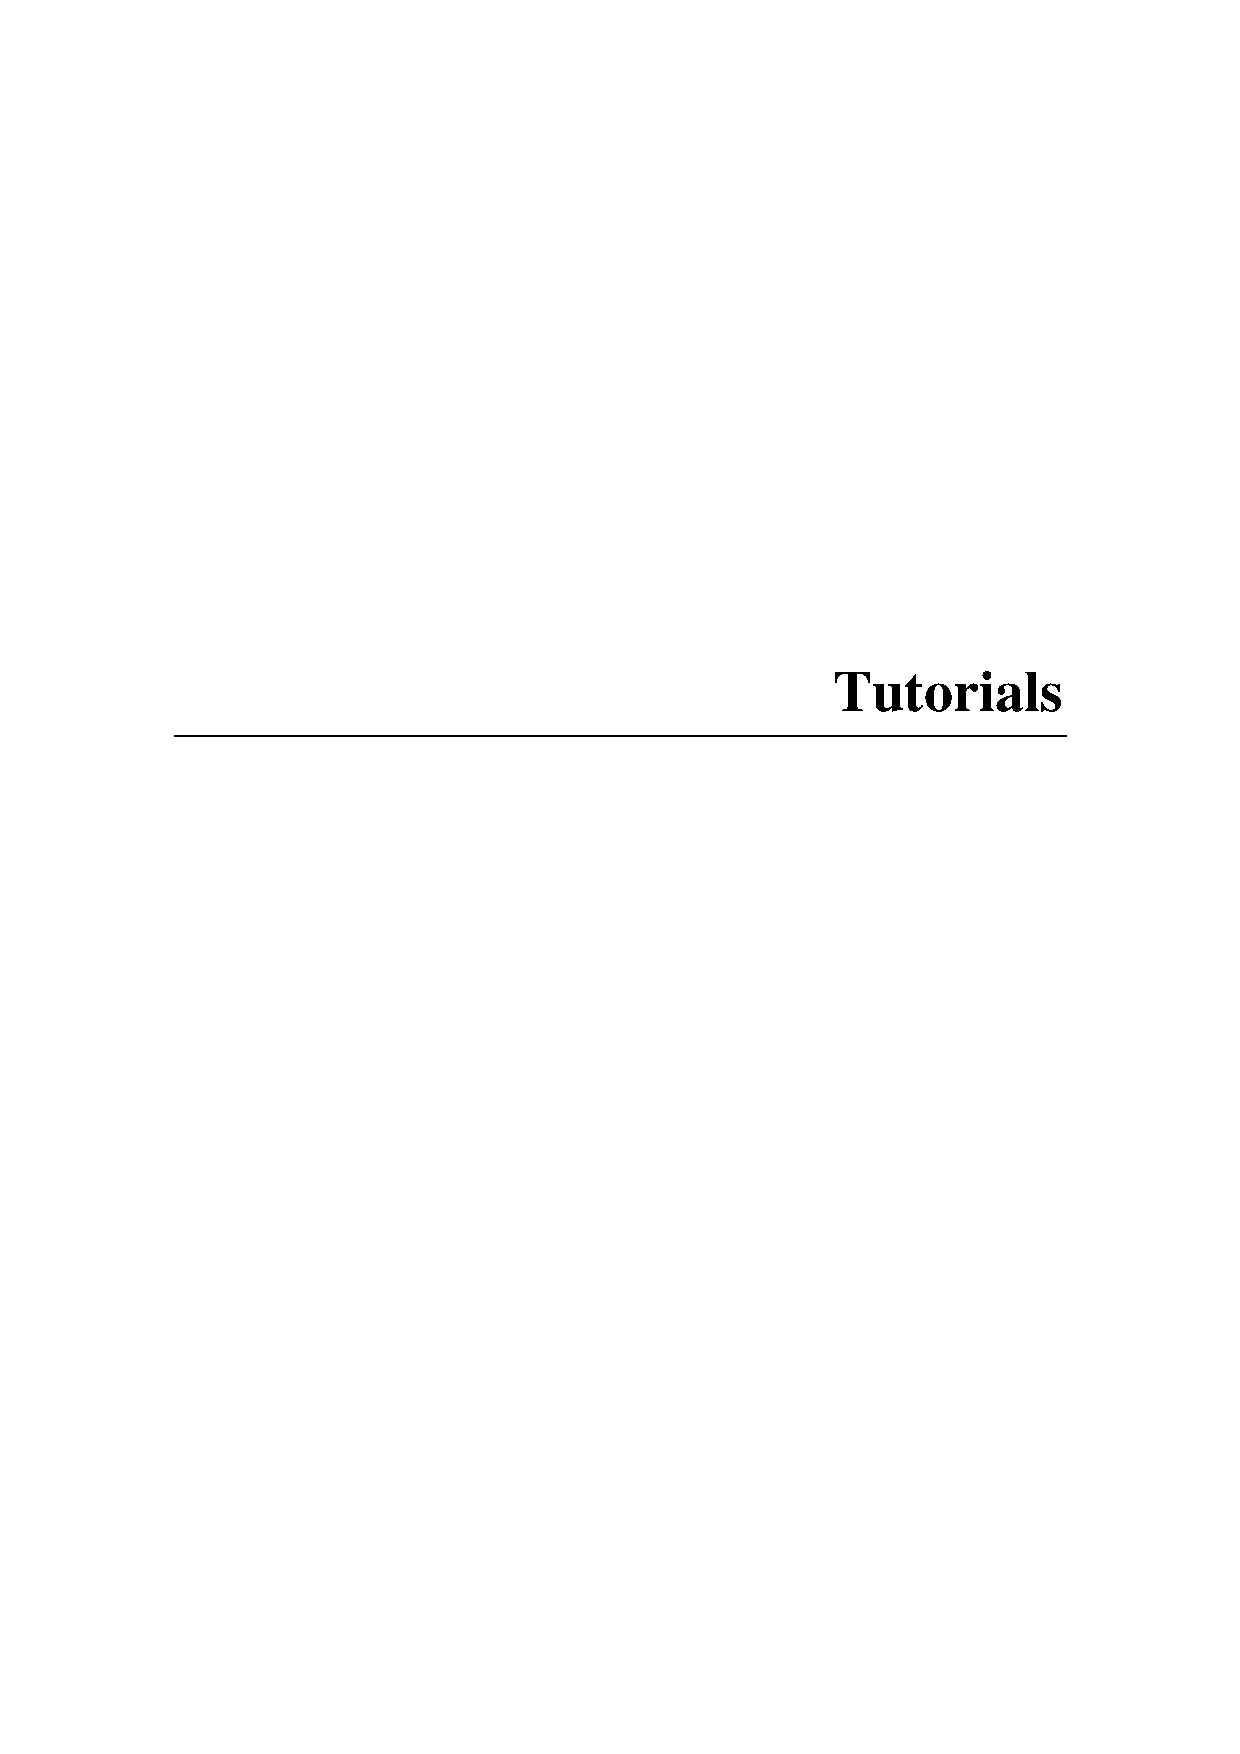
\includepdf[pages=1,pagecommand=\thispagestyle{empty}]{external/11_Tutorials.pdf}%
\thispagestyle{empty}\cleardoublepage
 %-------------------------------------------
% Tutorial 1
\includeabstract{Jazz solo analysis between music information
  retrieval, music psychology, and jazz research}{Jakob Abe{\ss}er,
  Klaus Frieler, Wolf-Georg Zaddach}{The tutorial will consist of four parts. The first part sets the scene with a short run through jazz history and its main styles and an overview of the central musical elements in jazz. Out of this introduction, the main research questions will be derived, which cover jazz research and jazz historiography, analysis of musical style, performance research, and psychology of creative processes. Particularly, research issues as addressed in the Jazzomat Research Project will be discussed and results will be presented.

The second part of the tutorial will deal with the details of the Weimar Jazz Database. Each solo encompasses pitch, onset, and offset time of the played tones as well as several additional annotations, e.g., manually tapped beat grids, chords, enumerations of sections and choruses as well as phrase segmentations. The process of creating the monophonic transcriptions will be explained (solo selection, transcription procedure, and quality management) and examples will be shown. Moreover, the underlying data-model of the Weimar Jazz Database, which includes symbolic data as well as data automatically extracted from the audio-files (e.g., intensity curves and beat-wise bass chroma) will be discussed in detail.

In the third part, we will introduce our analysis tools MeloSpySuite and MeloSpyGUI, which allow the computation of a large set of currently over 500 symbolic features from monophonic melodies. These features quantify various tonal, harmonic, rhythmic, metrical, and structural properties of the solo melodies. In addition, pattern retrieval modules, based on n-gram representations and a two-stage search option using regular expressions, play an integral part for the extraction of motivic cells and formulas from jazz solos. All tools can be readily applied to other melodic datasets besides the Weimar Jazz Database. Several use cases will be demonstrated and research results will be discussed.

The final part of the tutorial will focus on audio-based analysis of recorded jazz solo performances. We follow a score-informed analysis approach by using the solo transcriptions from the Weimar Jazz Database as prior information. This allows us to mitigate common problems in transcribing and analyzing polyphonic and multi-timbral audio such as overlapping instrument partials. A score-informed source separation algorithm is used to split the original recordings into a solo and an accompaniment track, which allows the tracking of f0-curves and intensity contours of the solo instrument. We will present the results of different analyses of the stylistic idiosyncrasies across well-known saxophone and trumpet players. Finally, we will briefly outline further potentials and challenges of score-informed MIR techniques.}{\paragraph{Jakob Abeßer} holds a degree in computer engineering (Dipl.-Ing.) from Ilmenau University of Technology. He is a postdoctoral researcher in the Semantic Music Technologies group at Fraunhofer IDMT and obtained a PhD degree (Dr.-Ing.) in Media Technology from Ilmenau University of Technology in 2014. During his PhD, he was a visiting researcher at the Finnish Centre of Excellence in Interdisciplinary Music Research, University of Jyväskylä, Finland in 2010. As a research scientist at Fraunhofer, he has experience with algorithm development in the fields of automatic music transcription, symbolic music analysis, machine learning, and music instrument recognition. Also, he works as a postdoctoral researcher at the University of Music in Weimar in the Jazzomat Research Project, focusing on analyzing jazz solo recordings using Music Information Retrieval technologies.

\paragraph{Klaus Frieler} graduated in theoretical physics (diploma) and received a PhD in systematic musicology in 2008. In between, he worked several years as a freelance software developer before taking up a post as lecturer in systematic musicology at the University of Hamburg in 2008. In 2012, he had a short stint at the C4DM, Queen Mary University of London. Since the end of 2012, he is a post-doctoral researcher with the Jazzomat Research Project at the University of Music “Franz Liszt” Weimar. His main research interests are computational and statistical music psychology with a focus on creativity, melody perception, singing intonation, and jazz research. Since 2006, he also works as an independent music expert specializing in copyright cases.

\paragraph{Wolf-Georg Zaddach} studied musicology, arts administration, and history in Weimar and Jena, music management and jazz guitar in Prague, Czech Republic. After finishing his Magister Artium with a thesis about jazz in Czechoslovakia in the 50s and 60s, he worked as assistant professor at the department of musicology in Weimar. Since 10/2012 he works at the jazz research project of Prof. Dr. Martin Pfleiderer. Since 02/2014, he holds a scholarship by the German National Academic Foundation (Studienstiftung des deutschen Volkes) for his Ph.D. about heavy and extreme metal in the 1980s GDR/East Germany. He frequently performs live and on records as a guitarist.}

% Tutorial 2
\includeabstract{Music Information Retrieval: Overview, Recent
  Developments and Future Challenges}{Emilia G\'omez, Markus Schedl,
  Xavier Serra, Xiao Hu}{This tutorial provides a survey of the field of Music Information Retrieval (MIR), that aims, among other things, at automatically extracting semantically meaningful information from various representations of music entities, such as audio, scores, lyrics, web pages or microblogs. The tutorial is designed for students, engineers, researchers, and data scientists who are new to MIR and want to get introduced to the field.

The tutorial will cover some of the main tasks in MIR, such as music identification, transcription, search by similarity, genre/mood/artist classification, query by humming, music recommendation, and playlist generation. We will review approaches based on content-based and context-based music description and show how MIR tasks are addressed from a user-centered and multicultural perspective. The tutorial will focus on latest developments and current challenges in the field.}{\paragraph{Emilia Gómez} is an Associate Professor (Serra-Hunter Fellow) at the Music Technology Group, Department of Information and Communication Technologies, Universitat Pompeu Fabra in Barcelona, Spain. She graduated as a Telecommunication Engineer at Universidad de Sevilla (Spain) and she studied classical piano performance at Seville Conservatoire of Music. She then received a DEA in Acoustics, Signal Processing and Computer Science applied to Music (ATIAM) at IRCAM, Paris (France) and a Ph.D. in Computer Science and Digital Communication at the UPF (awarded by EPSON foundation). Her research is within the Music Information Retrieval (MIR) field. She tries to understand and enhance music listening experiences by automatically extracting descriptors from music signals. She has designed algorithms able to describe music signals in terms of melody, tonality, and, by incorporating machine learning techniques, she has been able to model high-level concepts such as similarity, style or emotion. Emilia Gómez has co-authored more than a 100 publications in peer-reviewed scientific journals and conferences. She has contributed to more than 15 research projects, most of them funded by the European Commission and Spanish Government. She is elected member-at-large of the International Society for Music Information Retrieval (ISMIR). At the moment, she contributes to the COFLA project on computational analysis of flamenco music and she is the principal investigator for the European research project PHENICX, trying to innovate the way we experience classical music concerts.

\paragraph{Markus Schedl} is an Associate Professor at the Johannes Kepler University Linz / Department of Computational Perception. He graduated in Computer Science from the Vienna University of Technology and earned his Ph.D. in Technical Sciences from the Johannes Kepler University Linz. Markus further studied International Business Administration at the Vienna University of Economics and Business Administration as well as at the Handelshogskolan of the University of Gothenburg, which led to a Master’s degree. Markus (co-)authored more than 120 refereed conference papers and journal articles (among others, published in ACM Multimedia, SIGIR, ECIR, IEEE Visualization; Journal of Machine Learning Research, ACM Transactions on Information Systems, Springer Information Retrieval, IEEE Multimedia). Furthermore, he is associate editor of the Springer International Journal of Multimedia Information Retrieval and serves on various program committees and reviewed submissions to several conferences and journals (among others, ACM Multimedia, ECIR, IJCAI, ICASSP, IEEE Visualization; IEEE Transactions of Multimedia, Elsevier Data \& Knowledge Engineering, ACM Transactions on Intelligent Systems and Technology, Springer Multimedia Systems). His main research interests include web and social media mining, information retrieval, multimedia, and music information research. Since 2007, Markus has been giving several lectures, among others, ”Music Information Retrieval”, ”Exploratory Data Analysis”, ”Multimedia Search and Retrieval”, ”Learning from User-generated Data”, ”Multimedia Data Mining”, and ”Intelligent Systems”. He further spent several guest lecturing stays at the Universitat Pompeu Fabra, Barcelona, Spain, the Utrecht University, the Netherlands, the Queen Mary, University of London, UK, and the Kungliga Tekniska Hgskolan, Stockholm, Sweden.

\paragraph{Xavier Serra} is Associate Professor of the Department of Information and Communication Technologies and Director of the Music Technology Group at the Universitat Pompeu Fabra in Barcelona. After a multidisciplinary academic education he obtained a PhD in Computer Music from Stanford University in 1989 with a dissertation on the spectral processing of musical sounds that is considered a key reference in the field. His research interests cover the analysis, description and synthesis of sound and music signals, with a balance between basic and applied research and approaches from both scientific/technological and humanistic/artistic disciplines. Dr. Serra is very active in promoting initiatives in the field of Sound and Music Computing at the local and international levels, being involved in the editorial board of a number of journals and conferences and giving lectures on current and future challenges of the field. He has recently been awarded an Advanced Grant of the European Research Council to carry out the project CompMusic aimed at promoting multicultural approaches in music computing research.

\paragraph{Xiao Hu} is an Assistant Professor in the Division of Information and Technology Studies in the Faculty of Ed- ucation of the University of Hong Kong. She received her Ph.D degree in Library and Information Science from the University of Illinois, with an award winning dissertation on multimodal music mood classification. Dr. Hu’s research interests include music mood recognition, MIR evaluation, user-centered MIR studies and cross-cultural MIR. Dr. Hu has won the Best Student Paper award in the ACM Joint Conference on Digital Libraries (2010) and Best Student Paper award in the iConference (2010). Dr. Hu has been a visiting scholar at the National Institute of Informatics, Japan. She was a tutorial speaker on music affect recognition (2012) and a Conference Co-chair (2014) in the International Society for Music Information Retrieval Conference.}
%  Xavier Serra, Xiao Hu}{external/11-2_Tutorial-2.pdf}{}

% Tutorial 3
\includeabstract{Why is studio production interesting?}{Emmanuel
  Deruty, Fran\c{c}ois Pachet}{The tutorial follows the “Why X is interesting” series that aims at bridging the gap between technology-oriented and music-related research. It will suggest a number of reasons why production is important for MIR, seen from the eyes of an expert (the first author) and a MIR researcher (the second one).

In music, the use of studio techniques has become commonplace with the advent of cheap personal computers and powerful DAWs. The MIR community has long been confronted to studio production. Since ISMIR’s first installment in 2000, about 35 papers involving more than 70 authors have addressed studio production. However, more than 44% of these identify studio production as a source of problems: the so-called album or producer effect gets in the way of artist or genre identification, audio processing techniques prevent proper onset detections, or effects are responsible for false positive in singing voice detection. A few of these papers even characterize production as not being part of the music. On the other hand, another 35% of these papers either outline the knowledge of studio production as useful or indispensable to MIR tasks, or try to provide a formal characterization for this set of techniques.

A difficulty met by MIR researchers interested in studio production techniques is that production specialists are reluctant to formalize their knowledge. Like old-fashioned guild artisans, engineers and producers reputedly learn “tricks of the trade” from the “Greatest Teachers” or “mentors”. As a result, knowledge of studio production techniques is not widespread in the scientific community. Even in the upcoming field of automatic mixing, a domain intrinsically related to studio production, we have found that only 15% of scientific papers take these techniques into account. A similar issue can be observed at DAFx, where papers dealing with studio production as actually performed in the music community are rare.

The tutorial aims at explaining studio production techniques to MIR researchers in a simple and practical way, in order to highlight the main production tricks and usages to a MIR audience.

We will review standard aspects of studio music production, including recording, processing, mixing, and mastering. We will then focus on the basic methods of audio processing: EQs, compression, reverbs, and such. We will illustrate how these basic techniques can be combined creatively.

Production techniques may be implemented in a variety of ways, depending on trends and available hardware. We’ll go through a brief retrospective of how these techniques have been used since the mid 60’s in different ways. As different variations of the same basic processes can influence, sometimes drastically, the finished product, we believe such knowledge may be useful in relation to classification and similarity.

MIR researchers often conceptualize lead vocals as a solo line, possibly ornamented with backing vocals and audio effects. In practice, we’ll show that vocal track production in mainstream pop music results in complex architectures. We will analyze the vocals tracks in some mainstream hits. It will demonstrate that studio production is an integral part of the music, not an extraneous layer of effects. Consequences are obvious for the nature of the information MIR scholars look for, e.g. in information extraction, retrieval, similarity or recommendation.

We will complete the tutorial with a short demo of automatic mixing techniques developed in our lab that use auto-adaptive audio effects. It will demonstrate that consideration of production is a definite advantage in music generation.}{\paragraph{Emmanuel Deruty} studied studio production for music at the Conservatoire de Paris (CNSMDP), where he graduated as Tonmeister in 2000. He has worked in many fields related to audio and music production in Europe and in the US: sound designer in a research context (IRCAM), sound designer in a commercial context (Soundwalk collective), film music producer and composer (Autour de Minuit \& Everybody on Deck, Paris), lecturer at Alchemea College of sound engineering (London), writer for the Sound on Sound magazine (Cambridge, UK). He’s worked as a M.I.R. researcher at IRCAM, INRIA and Akoustic-Arts, France. He’s currently working on automatic mixing at Sony CSL, and is a specialist of the “loudness war”.

\paragraph{François Pachet} received his Ph.D. and Habilitation degrees from Paris 6 University (UPMC). He is a Civil Engineer and was Assistant Professor in Artificial Intelligence and Computer Science, at Paris 6 University, until 1997. He is now director of the Sony Computer Science Laboratory in Paris, where he conducts research in interactive music listening and performance and musical metadata and developed several innovative technologies and award winning systems. François Pachet has published intensively in artificial intelligence and computer music. He was co-chair of the IJCAI 2015 special track on Artificial Intelligence and the Arts, and has been elected ECCAI Fellow in 2014. His current goal, funded by an ERC Advanced Grant, is to build computational representations of style from text and music corpora,that can be exploited for personalized content generation. He is also an accomplished musician (guitar, composition) and has published two music albums (in jazz and pop) as composer and performer.}
%  Deruty, Fran\c{c}ois Pachet}{external/11-3_Tutorial-3.pdf}{}

% Tutorial 4
\includeabstract{Introduction to EEG Decoding for Music Information Retrieval
Research}{Sebastian Stober, Blair Kaneshiro}{Perceptual and cognitive approaches to MIR research have very recently expanded to the realm of neuroscience, with MIR groups beginning to conduct neuroscience research and vice versa. First publications have already reached ISMIR and for the very first time, there will be a dedicated satellite event on cognitively based music informatics research (CogMIR) at this year’s ISMIR conference. Within the context of this growing potential for cross-disciplinary collaborations, this tutorial will provide fundamental knowledge of neuroscientific approaches and findings with the goal of sparking the interest of MIR researchers and leading to future intersections between these two exciting fields. Specifically, our focus for this tutorial is on electroencephalography (EEG), a widely used and relatively inexpensive recording modality which offers high temporal resolution, portability, and mobility – characteristics that may prove especially attractive for applications in MIR. Attendees of this tutorial will gain a fundamental understanding of EEG responses, including how the data are recorded as well as standard procedures for preprocessing and cleaning the data. Keeping in mind the interests and objectives of the MIR community, we will highlight EEG analysis approaches, including single-trial analyses, that lend themselves to retrieval scenarios. Finally, we will review relevant open-source software, tools, and datasets for facilitating future research. The tutorial will be structured as a combination of informational slides and live-coding analysis demonstrations, with ample time for Q\&A with the audience.}{\paragraph{Sebastian Stober} is head of the recently established junior research group on “Machine Learning in Cognitive Science” within the inter-disciplinary setting of the Research Focus Cognitive Science at the University of Potsdam. Before, he was a post-doctoral fellow at the Brain and Mind Institute of the University of Western Ontario where he investigated ways to identify perceived and imagined music pieces from electroencephalography (EEG) recordings. He studied computer science with focus on intelligent systems and music information retrieval at the Otto-von-Guericke University Magdeburg where he received his diploma degree in 2005 and his Ph.D. in 2011 for his thesis on adaptive methods for user-centered organization of music collections. He has also been co-organizer for the International Workshops on Learning Semantics of Audio Signals (LSAS) and Adaptive Multimedia Retrieval (AMR). With his current research on music imagery information retrieval, he combines music information retrieval with cognitive neuroscience.

\paragraph{Blair Kaneshiro} is a Ph.D. candidate (ABD) at the Center for Computer Research in Music and Acoustics at Stanford University. She earned her B.A. in Music, M.A. in Music, Science, and Technology, and M.S. in Electrical Engineering, all from Stanford. Her research explores musical engagement and expectation through brain responses, with an emphasis on multivariate and single-trial approaches to EEG analysis. Other research interests include the study of musical engagement using behavioral and large-scale social-media data, and promotion of reproducible and cross-disciplinary research through open-source tools and datasets. She is affiliated with CCRMA’s Music Engagement Research Initiative (MERI) led by professor Jonathan Berger; music tech company Shazam; and the Brain Research group (formerly Suppes Brain Lab) at Stanford’s Center for the Study of Language and Information.}
%Research}{Sebastian Stober, Blair Kaneshiro}{external/11-4_Tutorial-4.pdf}{}

% Tutorial 5
\includeabstract{Natural Language Processing for MIR}{Sergio Oramas,
  Luis Espinosa-Anke, Shuo Zhang, Horacio Saggion}{An increasing amount of musical information is being published daily in media like Social Networks, Digital Libraries or Web Pages. All this data has the potential to impact in musicological studies, as well as tasks within MIR such as music recommendation. Making sense of it is a very challenging task, and so this tutorial aims to provide the audience with potential applications of Natural Language Processing (NLP) to MIR and Computational Musicology.

In this tutorial, we will focus on linguistic, semantic and statistical­based approaches to extract and formalize knowledge about music from naturally occurring text. We propose to provide the audience with a preliminary introduction to NLP, covering its main tasks along with the state­of­the­art and most recent developments. In addition, we will showcase the main challenges that the music domain poses to the different NLP tasks, and the already developed methodologies for leveraging them in MIR and musicological applications. We will cover the following NLP tasks:

\begin{itemize}
\item Basic text preprocessing and normalization
\item Linguistic enrichment in the form of part­of­speech tagging, as well as shallow and dependency parsing.
\item Information Extraction, with special focus on Entity Linking and Relation Extraction.
\item Text Mining
\item Topic Modeling
\item Sentiment Analysis
\item Word Vector Embeddings
\end{itemize}

We will also introduce some of the most popular python libraries for NLP (e.g. Gensim, Spacy) and useful lexical resources (e.g. WordNet, BabelNet). At the same time, the tutorial analyzes the challenges and opportunities that the application of these techniques to large amounts of texts presents to MIR researchers and musicologists, presents some research contributions and provides a forum to discuss about how address those challenges in future research. We envisage this tutorial as a highly interactive session, with a sizable amount of hands­-on activities and live demos of actual systems.}{\paragraph{Sergio Oramas} received a degree in Computer Engineering by the Technical University of Madrid in 2004, and a B.A. in Musicology by the University of La Rioja in 2011. He is a PhD candidate at the Music Technology Group (Pompeu Fabra University) since 2013, holding a “La Caixa” PhD Fellowship. His research interests are focused on the extraction of structured knowledge from text and its application in Music Information Retrieval and Computational Musicology.

\paragraph{Luis Espinosa-Anke} is a PhD candidate at the Natural Language Processing group in at Pompeu Fabra University. His research focuses in learning knowledge representations of language, including automatic construction of glossaries; knowledge base generation, population and unification; and automatic taxonomy learning. He is Fulbright alumni, “laCaixa” scholar, and member of the Erasmus Mundus Association as well as the European Network of eLexicography.

\paragraph{Shuo Zhang} is a PhD candidate in Computational Linguistics at Georgetown University, USA, and a collaborator/researcher at the Music Technology Group, Universitat Pompeu Fabra. He has worked in both text (NLP­information extraction) and sound (speech processing­time­series data mining in speech prosody) aspects of computational linguistics and their applications in MIR. His past and current projects include areas such as coreference resolution, search and visualization of multilayered linguistic corpora, text mining \& topic modeling in MIR, temporal semantics, time­series mining in speech and music, etc. Shuo holds B.Sci. from the Peking University, M.A. from the Department of Music, University of Pittsburgh, and M.Sci. in Computational Linguistics from Georgetown University.

\paragraph{Horacio Saggion} is Profesor Agregado at the Department of Technologies, Universitat Pompeu Fabra. He holds a PhD in Computer Science from Université de Montréal (Canada). He is associated to the Natural Language Processing group where he works on automatic text summarization, text simplification, information extraction, text processing in social media, sentiment analysis and related topics. His research is empirical combining symbolic, pattern­based approaches and statistical and machine learning techniques. Before joining Universitat Pompeu Fabra, he worked at the University of Sheffield for a number of UK and European research projects developing competitive human language technology. He was also an invited researcher at Johns Hopkins University in 2011. Horacio has published over 100 works in leading scientific journals, conferences, and books in the field of human language technology.}
%  Luis Espinosa-Anke, Shuo Zhang, Horacio Saggion}{external/11-5_Tutorial-5.pdf}{}

% Tutorial 6
\includeabstract{Why Hip-Hop is interesting}{Jan Van Balen, Ethan
  Hein, Dan Brown}{Hip-hop, as a musical culture, is extremely popular around the world. Its influence on popular music is unprecedented: the hip-hop creative process has become the dominant practice of the pop mainstream, and spawned a range of electronic styles. Strangely, Hip-hop hasn’t been the subject of much research in Music Information Retrieval. Music research rooted in the European music traditions tends to look at music in terms harmony, melody and form. Even compared to other popular music, these are facets of music that don’t quite work the same way in Hip-Hop as they do in the music of Beethoven and the Beatles.

In this tutorial, we will argue that a different perspective may be needed to approach the analysis of Hip-hop and popular music computationally—an analysis with a stronger focus on timbre, rhythm and lyrics and attention to groove, texture, rhyme, metadata and semiotics.

Hip-hop is often said to integrate four modes of artistic expression: Rap, turntablism, breakdance and graffiti culture. In the first part of this tutorial, we will discuss the emergence and evolution of Hip-Hop as a musical genre, and its particularities, focusing our discussion on beat-making (turntablism and sampling), and Rap. A second part of the talk will highlight the most important reasons why MIR practitioners and other music technologists should care about Hip-Hop, talking about Hip-hop’s relevance today, and the role Hip-hop in popular music. We highlight its relative absence in music theory, music education, and MIR. The latter will be illustrated with examples of MIR and digital musicology studies in which Hip-hop music is explicitly ignored or found to ‘break’ the methodology.

Next, we review some of the work done on the intersection of Hip-hop and music technology. Because the amount of computational research on Hip-hop music is rather modest, we discuss, in depth, three clusters of research on the intersection of Hip-hop and music technology. The first two are related of MIR, focusing on ‘beats’ and sampling, and Rap lyrics and rhyme. For the third topic, situating Hip-hop in the broader topic of music technology, we look at how an important role for both music technology and Hip-hop is emerging in music education. Finally, the last part of the talk will give an overview of resources and research opportunities for Hip-hop research.

This tutorial is aimed at anyone interested in Music Information Retrieval and popular music, whether familiar with Hip-hop music or not. We also aim to make it relevant to a broader audience interested in music technology, touching on topics like sampling and samplers, and Hip-hop in technology and music education, and to anyone interested in text processing, with an additional focus on the analysis of lyrics.

Throughout the tutorial, we intend to include a lot of listening examples. Participants will access to an extended playlist of selected listening examples, along with a short guide to the significance of the selected recordings.}{\paragraph{Jan Van Balen} researches the use of audio MIR methods to learn new things about music and music memory. Living in London, he is finishing his PhD with Utrecht University (NL), on audio corpus analysis and popular music. As part of his PhD project and with colleagues at Utrecht University and University of Amsterdam, he worked on Hooked, a game to collect data on popular music memory and ‘hooks’. Other work has focused on the analysis of the game’s audio and participant data, and on content ID techniques for the analysis of samples, cover songs and folk tunes.

\paragraph{Ethan Hein} is a doctoral student in music education at New York University. He teaches music technology, production and education at NYU and Montclair State University. As the Experience Designer In Residence with the NYU Music Experience Design Lab, Ethan has taken a leadership role in a range of technologies for learning and expression. In collaboration with Soundfly, he recently launched an online course called Theory For Producers. He maintains a widely-followed and influential blog at http://www.ethanhein.com, and has written for various publications, including Slate, Quartz, and NewMusicBox.

\paragraph{Dan Brown} is Associate Professor of Computer Science at the University of Waterloo, where he has been a faculty member since 2000. Dan earned his Bachelor’s degree in Math with Computer Science from MIT, and his PhD in Computer Science from Cornell. Before coming to Waterloo, he spent a year working on the Human and Mouse Genome Projects as a post-doc at the MIT Center for Genome Research. Dan’s primary research interests are designing algorithms for understanding biological evolution, and applying bioinformatics ideas to problems in music information retrieval.}
%  Hein, Dan Brown}{external/11-6_Tutorial-6.pdf}{}
